\documentclass[11pt,a4paper]{article}
\usepackage[utf8]{inputenc}
\usepackage[T1]{fontenc}
\usepackage{lmodern}
\usepackage[portuguese]{babel}
\usepackage[a4paper,margin=2.4cm]{geometry}
\usepackage{xcolor}
\usepackage{graphicx}
\usepackage{titlesec}
\usepackage{enumitem}
\usepackage{listings}
\usepackage{tcolorbox}
\usepackage{booktabs}
\usepackage{array}
\usepackage{fancyhdr}
\usepackage{hyperref}
\tcbuselibrary{skins,breakable,listings}

\definecolor{BgCream}{HTML}{FAF8F5}
\definecolor{TextEspresso}{HTML}{4A4238}
\definecolor{NudeTaupe}{HTML}{BFAFA6}
\definecolor{SoftBlush}{HTML}{D9C5B2}
\definecolor{SageMuted}{HTML}{7E8F7C}
\definecolor{ClayWarn}{HTML}{B5795C}
\definecolor{SkyCalm}{HTML}{5E7F9A}

\hypersetup{colorlinks=true, linkcolor=SkyCalm, urlcolor=SkyCalm}

\titleformat{\section}{\color{TextEspresso}\Large\bfseries}{\thesection}{0.6em}{}[{\color{NudeTaupe}\titlerule[0.8pt]}]
\titlespacing*{\section}{0pt}{1.6\baselineskip}{0.9\baselineskip}

\setlength{\parindent}{0pt}
\setlength{\parskip}{0.5cm}
\linespread{1.18}
\setlist[itemize]{itemsep=0.3cm, topsep=0.3cm}
\setlist[enumerate]{itemsep=0.3cm, topsep=0.3cm}

\pagestyle{fancy}
\fancyhf{}
\renewcommand{\headrulewidth}{0pt}
\fancyfoot[C]{\color{NudeTaupe}\small\thepage}

% Terminal: fundo preto, letra branca
\newtcblisting{terminal}{
  listing only, breakable, colback=black, colupper=white, colframe=TextEspresso,
  boxrule=0.8pt, arc=3pt, left=10pt, right=10pt, top=8pt, bottom=8pt,
  before skip=0.45cm, after skip=0.6cm,
  title={\small\bfseries Comando a executar},
  coltitle=white, colbacktitle=TextEspresso, fonttitle=\small\bfseries,
  listing options={basicstyle=\ttfamily\small\color{white}, breaklines=true,
    columns=fullflexible, keepspaces=true, showstringspaces=false}
}

\newtcblisting{saida}{
  listing only, breakable, colback=black, colupper=white, colframe=SageMuted,
  boxrule=0.8pt, arc=3pt, left=10pt, right=10pt, top=8pt, bottom=8pt,
  before skip=0.45cm, after skip=0.6cm,
  title={\small\bfseries Resultado esperado (os valores podem variar)},
  coltitle=white, colbacktitle=SageMuted, fonttitle=\small\bfseries,
  listing options={basicstyle=\ttfamily\footnotesize\color{white}, breaklines=true,
    columns=fullflexible, keepspaces=true, showstringspaces=false}
}

\newtcblisting{ficheiro}[1]{
  listing only, breakable, colback=BgCream, colupper=TextEspresso, colframe=SkyCalm,
  boxrule=0.8pt, arc=3pt, left=10pt, right=10pt, top=8pt, bottom=8pt,
  before skip=0.45cm, after skip=0.6cm,
  title={\small\bfseries Conteúdo do ficheiro \texttt{#1}},
  coltitle=white, colbacktitle=SkyCalm, fonttitle=\small\bfseries,
  listing options={basicstyle=\ttfamily\small\color{TextEspresso}, breaklines=true,
    columns=fullflexible, keepspaces=true, showstringspaces=false}
}

\newtcolorbox{erro}{
  breakable, colback=ClayWarn!9, colframe=ClayWarn, boxrule=0.8pt, arc=3pt,
  left=10pt, right=10pt, top=8pt, bottom=8pt, before skip=0.5cm, after skip=0.6cm,
  title={\small\bfseries Erro possível e resolução},
  coltitle=white, colbacktitle=ClayWarn, fonttitle=\small\bfseries
}

\newtcolorbox{observe}{
  breakable, colback=SoftBlush!30, colframe=NudeTaupe, boxrule=0.8pt, arc=3pt,
  left=10pt, right=10pt, top=8pt, bottom=8pt, before skip=0.5cm, after skip=0.6cm,
  title={\small\bfseries Analisar},
  coltitle=TextEspresso, colbacktitle=SoftBlush, fonttitle=\small\bfseries
}

\newtcolorbox{nota}{
  breakable, colback=SkyCalm!8, colframe=SkyCalm, boxrule=0.8pt, arc=3pt,
  left=10pt, right=10pt, top=8pt, bottom=8pt, before skip=0.5cm, after skip=0.6cm,
  title={\small\bfseries Nota},
  coltitle=white, colbacktitle=SkyCalm, fonttitle=\small\bfseries
}

\newtcolorbox{feito}{
  breakable, colback=SageMuted!10, colframe=SageMuted, boxrule=0.8pt, arc=3pt,
  left=10pt, right=10pt, top=8pt, bottom=8pt, before skip=0.5cm, after skip=0.6cm,
  title={\small\bfseries Verificação antes de avançar},
  coltitle=white, colbacktitle=SageMuted, fonttitle=\small\bfseries
}

\newtcolorbox{leitura}{
  breakable, colback=SkyCalm!6, colframe=SkyCalm, boxrule=0.8pt, arc=3pt,
  left=10pt, right=10pt, top=8pt, bottom=8pt, before skip=0.4cm, after skip=0.6cm,
  title={\small\bfseries Como ler a figura},
  coltitle=white, colbacktitle=SkyCalm, fonttitle=\small\bfseries
}

\newtcolorbox{teoria}{
  breakable, colback=BgCream, colframe=TextEspresso, boxrule=0.8pt, arc=3pt,
  left=12pt, right=12pt, top=10pt, bottom=10pt, before skip=0.5cm, after skip=0.7cm,
  title={\small\bfseries Fundamento teórico},
  coltitle=white, colbacktitle=TextEspresso, fonttitle=\small\bfseries,
  before upper={\setlength{\parskip}{0.35cm}}
}

\newcommand{\passo}[2]{%
  \clearpage
  \begin{tcolorbox}[colback=SageMuted, colframe=SageMuted, coltext=white,
    boxrule=0pt, arc=4pt, left=14pt, right=14pt, top=10pt, bottom=10pt,
    before skip=0pt, after skip=0.6cm]
  {\Large\bfseries Passo #1}\hfill{\large\bfseries #2}
  \end{tcolorbox}
}

\newcommand{\cmd}[1]{\texttt{#1}}

\newcommand{\labtitle}[3]{%
  \thispagestyle{empty}
  \begin{center}
  {\color{NudeTaupe}\rule{\textwidth}{0.5pt}}\\[0.6cm]
  {\LARGE\bfseries\color{TextEspresso} Laboratório #1}\\[0.4cm]
  {\large\color{TextEspresso} #2}\\[0.35cm]
  {\normalsize\color{NudeTaupe} Infraestruturas de Computação na Nuvem \quad|\quad #3}\\[0.5cm]
  {\color{NudeTaupe}\rule{\textwidth}{0.5pt}}
  \end{center}
  \vspace{0.5cm}
}

\begin{document}
\labtitle{06}{Primeiro Contacto com Redes Definidas por Software}{Aula 06}

\section*{Objetivo e enquadramento}

A Aula 06 apresenta, no plano teórico, a separação entre o plano de controlo e o plano de dados, o protocolo OpenFlow, as tabelas de fluxos e as redes overlay. Este laboratório torna esses conceitos observáveis numa rede virtual construída na máquina do próprio aluno, com o Mininet, o Open vSwitch e o controller Ryu.

O trabalho não requer acesso ao servidor da unidade curricular nem a qualquer serviço de nuvem. Destina-se a ser realizado durante a aula, ao ritmo de cada aluno, e \textbf{não constitui trabalho a entregar}. Todo o trabalho decorre numa máquina virtual Ubuntu, criada e apagada com um único comando, de modo que o computador do aluno permanece intacto.

\begin{nota}
O Mininet e o Open vSwitch exigem um núcleo Linux. Por esse motivo o laboratório utiliza uma máquina virtual criada com o \cmd{multipass}, que funciona da mesma forma em Windows, macOS e Linux. Quem utilizar Linux pode executar os passos diretamente no seu sistema, a partir do passo 1.3.
\end{nota}

\section*{Resultados de aprendizagem}

No final deste laboratório, o aluno deve ser capaz de:

\begin{itemize}
  \item Criar uma topologia virtual com hosts e um switch Open vSwitch.
  \item Demonstrar que um switch sem controller nem regras não encaminha tráfego.
  \item Ligar um controller Ryu e observar o modelo reativo, com mensagens \emph{packet-in}.
  \item Ler uma tabela de fluxos e identificar prioridade, contadores e \emph{timeouts}.
  \item Instalar uma regra de bloqueio e explicar a razão pela qual prevalece sobre as restantes.
  \item Criar um túnel VXLAN entre dois namespaces e observar o encapsulamento em UDP.
\end{itemize}

\section*{Requisitos}

\begin{itemize}
  \item Computador com Windows, macOS ou Linux.
  \item Cerca de 2 GB de memória livres para a máquina virtual e 10 GB de espaço em disco.
  \item Ligação à Internet, necessária para obter a imagem e os pacotes.
  \item Permissão para instalar o \cmd{multipass} (Windows e macOS) ou o \cmd{snap} (Linux).
  \item Duração estimada: entre 75 e 100 minutos.
\end{itemize}

\section*{Como utilizar este guião}

Cada passo apresenta, por esta ordem, o objetivo, o enquadramento, o fundamento teórico, os comandos a executar e o resultado esperado. Recomenda-se ler o passo completo antes de executar o primeiro comando. As caixas têm sempre o mesmo significado:

\begin{terminal}
Comando a executar no terminal.
\end{terminal}

\begin{saida}
Resultado que deve ser apresentado.
\end{saida}

\begin{observe}
Momento de pausa para interpretar o resultado obtido, isoladamente ou em discussão com os colegas.
\end{observe}

\begin{erro}
Erro que pode ocorrer e respetiva resolução.
\end{erro}

\begin{nota}
Informação complementar que facilita a execução.
\end{nota}

Os comandos podem ser copiados e colados. Os resultados mostrados são exemplos: endereços, contadores, tempos e números de versão diferem de computador para computador. O prompt \cmd{mininet>} indica que o comando é escrito na consola do Mininet, e não no terminal da máquina virtual.

\section*{Percurso}

A figura seguinte resume a sequência do guião. Os passos 3 e 4 constituem a observação central: um controller instala regras na tabela de fluxos de um switch, e essas regras são visíveis e mensuráveis.

\begin{center}
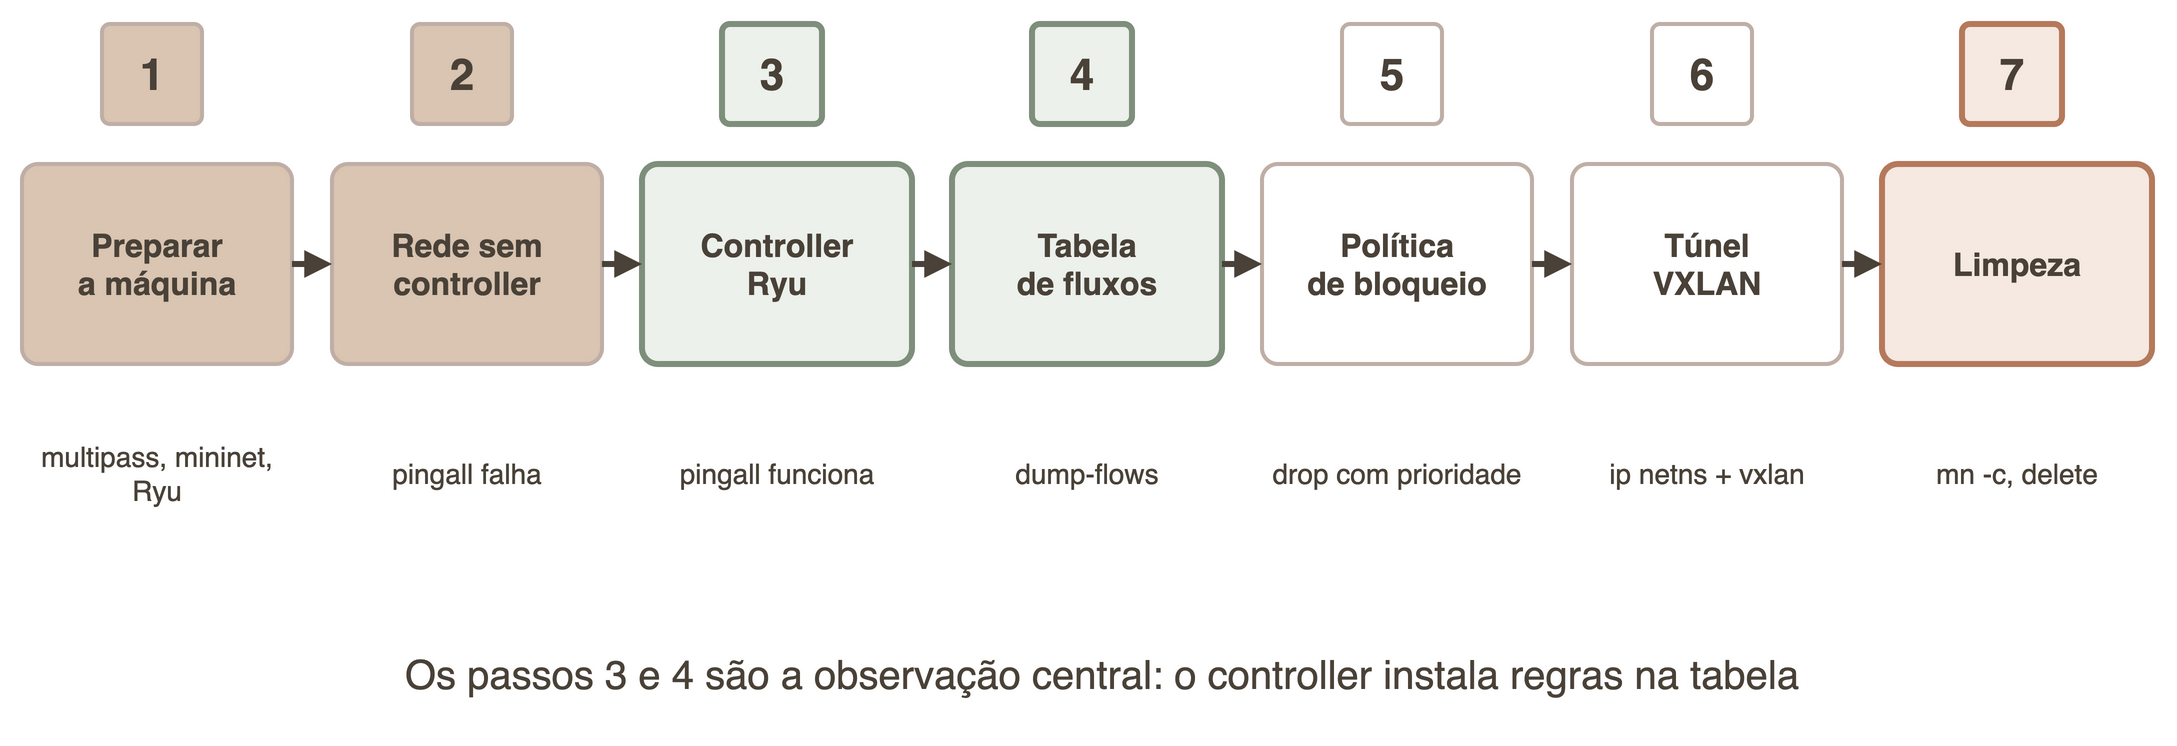
\includegraphics[width=\linewidth]{../Diagramas/g06-percurso.png}
\end{center}

\begin{leitura}
Os sete passos leem-se da esquerda para a direita. Os dois primeiros, a bege, preparam o ambiente e mostram o comportamento de uma rede sem controller. Os passos 3 e 4, a verde, são a parte central: liga-se o controller e lê-se a tabela de fluxos que ele construiu. Os passos 5 e 6, a branco, acrescentam uma política de bloqueio e um túnel VXLAN. O passo 7, em tom avermelhado, encerra o trabalho e liberta os recursos. Abaixo de cada caixa, uma legenda resume o que é feito nesse passo.
\end{leitura}

\passo{1}{Preparação do ambiente}

\textbf{Objetivo.} Criar uma máquina virtual Ubuntu e instalar nela o Mininet, o Open vSwitch e o controller Ryu.

\textbf{Enquadramento.} O Mininet emula hosts e switches num único sistema Linux, recorrendo aos namespaces de rede estudados na Aula 04. Cada host do Mininet é, na prática, um processo com a sua própria pilha de rede.

\begin{center}
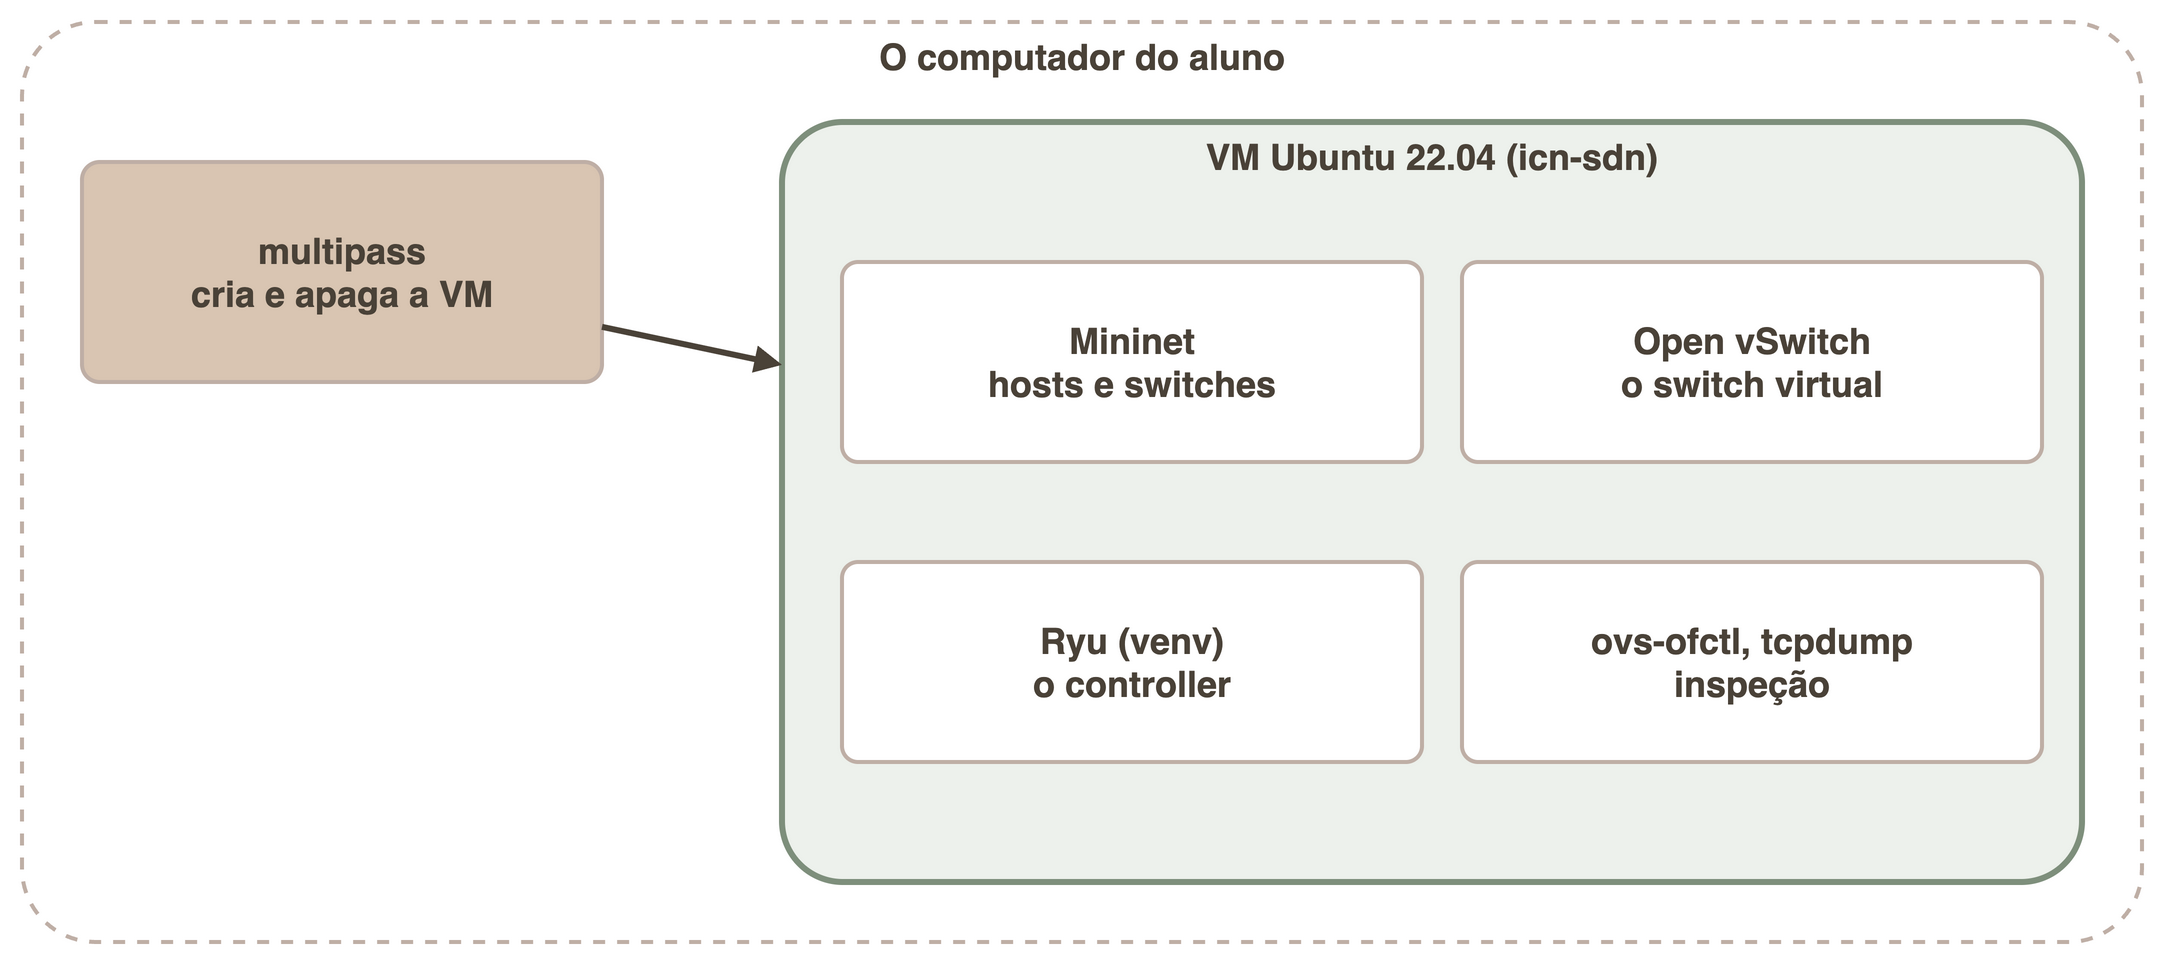
\includegraphics[width=\linewidth]{../Diagramas/g06-ferramentas.png}
\end{center}

\begin{leitura}
A caixa exterior representa o computador do aluno. À esquerda está o \cmd{multipass}, o único programa instalado no computador, cuja função é criar e apagar a máquina virtual. A caixa verde é essa máquina virtual. Dentro dela estão as quatro peças do laboratório: o Mininet, que cria a rede emulada, o Open vSwitch, que é o switch usado nessa rede, o Ryu, que é o controller, e as ferramentas de inspeção. Tudo o que é instalado fica dentro da máquina virtual e desaparece quando esta é apagada.
\end{leitura}

\begin{teoria}
O Mininet não simula uma rede: emula-a. Cada host é um processo comum do Linux, colocado num namespace de rede próprio, com uma interface virtual ligada por um par \emph{veth} ao switch. Os comandos que se executam num host correm, de facto, no núcleo real. Por isso o \cmd{ping} mede tráfego verdadeiro e o Open vSwitch utilizado é o mesmo que se encontra em hipervisores de produção.

O Ryu é um \emph{framework} em Python para escrever controllers OpenFlow. Cada aplicação reage a eventos, como a ligação de um switch ou a chegada de um \emph{packet-in}. Para ser executado de forma isolada, instala-se num ambiente virtual do Python, de modo a não interferir com os pacotes do sistema.

\textbf{A analisar neste passo:} onde vive cada ferramenta. Apenas o \cmd{multipass} corre no computador do aluno, e tudo o resto corre dentro da máquina virtual.
\end{teoria}

\subsection*{1.1 Instalação do Multipass}

Em macOS, com o Homebrew, executar o comando seguinte. Em Windows, utilizar o instalador disponível em \url{https://multipass.run}. Em Linux, o \cmd{multipass} instala-se com o \cmd{snap}.

\begin{terminal}
brew install --cask multipass
\end{terminal}

\begin{terminal}
sudo snap install multipass
\end{terminal}

O primeiro comando destina-se a macOS e o segundo a Linux. Confirmar a instalação:

\begin{terminal}
multipass version
\end{terminal}

\begin{saida}
multipass   1.xx.x
\end{saida}

\begin{erro}
\textbf{command not found}: fechar o terminal e abrir um novo. Em Windows, utilizar o PowerShell e confirmar que o instalador terminou sem erros.
\end{erro}

\subsection*{1.2 Criação da máquina virtual}

\begin{terminal}
multipass launch 22.04 --name icn-sdn --cpus 2 --memory 2G --disk 10G
multipass shell icn-sdn
\end{terminal}

\begin{saida}
Launched: icn-sdn
ubuntu@icn-sdn:~$
\end{saida}

A partir deste momento, todos os comandos são executados dentro da máquina virtual, no prompt \cmd{ubuntu@icn-sdn}. A primeira execução demora alguns minutos, por incluir a obtenção da imagem.

\begin{erro}
\textbf{launch failed} ou execução parada: o computador não dispõe de memória livre suficiente. Fechar outras aplicações e repetir. Se a máquina já existir, executar \cmd{multipass delete icn-sdn}, \cmd{multipass purge} e repetir.
\end{erro}

\subsection*{1.3 Instalação do Mininet, do Open vSwitch e das ferramentas}

\begin{terminal}
sudo apt update
sudo apt install -y mininet openvswitch-switch python3-venv tcpdump
\end{terminal}

Confirmar que o Open vSwitch e o Mininet respondem:

\begin{terminal}
sudo ovs-vsctl --version
sudo mn --version
\end{terminal}

\begin{saida}
ovs-vsctl (Open vSwitch) 2.17.x
2.3.x
\end{saida}

\subsection*{1.4 Instalação do Ryu}

O Ryu é instalado num ambiente virtual. O pacote \cmd{eventlet} é fixado numa versão antiga, porque as versões recentes são incompatíveis com o Ryu.

\begin{terminal}
mkdir -p ~/icn-aula06
python3 -m venv ~/ryu-env
~/ryu-env/bin/pip install ryu "eventlet==0.30.1"
~/ryu-env/bin/ryu-manager --version
\end{terminal}

\begin{saida}
ryu-manager 4.34
\end{saida}

\begin{erro}
\textbf{Falha na compilação do Ryu}, com mensagens sobre \cmd{setuptools}: instalar primeiro uma versão anterior do \cmd{setuptools}, com \cmd{\textasciitilde/ryu-env/bin/pip install "setuptools==58.2.0" wheel}, e repetir a instalação do Ryu.

\textbf{ImportError} sobre \cmd{ALREADY\_HANDLED} ao arrancar o \cmd{ryu-manager}: o \cmd{eventlet} instalado é demasiado recente. Executar \cmd{\textasciitilde/ryu-env/bin/pip install "eventlet==0.30.1"}.
\end{erro}

\begin{feito}
Os comandos \cmd{sudo ovs-vsctl -{}-version}, \cmd{sudo mn -{}-version} e \cmd{\textasciitilde/ryu-env/bin/ryu-manager -{}-version} executam sem erro.
\end{feito}

\passo{2}{Uma rede sem controller}

\textbf{Objetivo.} Criar uma topologia com três hosts e um switch, e demonstrar que, sem controller e sem regras, o switch não encaminha tráfego.

\textbf{Enquadramento.} Na Aula 06, o plano de dados foi apresentado como a parte que aplica regras já instaladas. Se não houver regras, o plano de dados não tem critério para decidir. Este passo mostra esse efeito.

\begin{center}
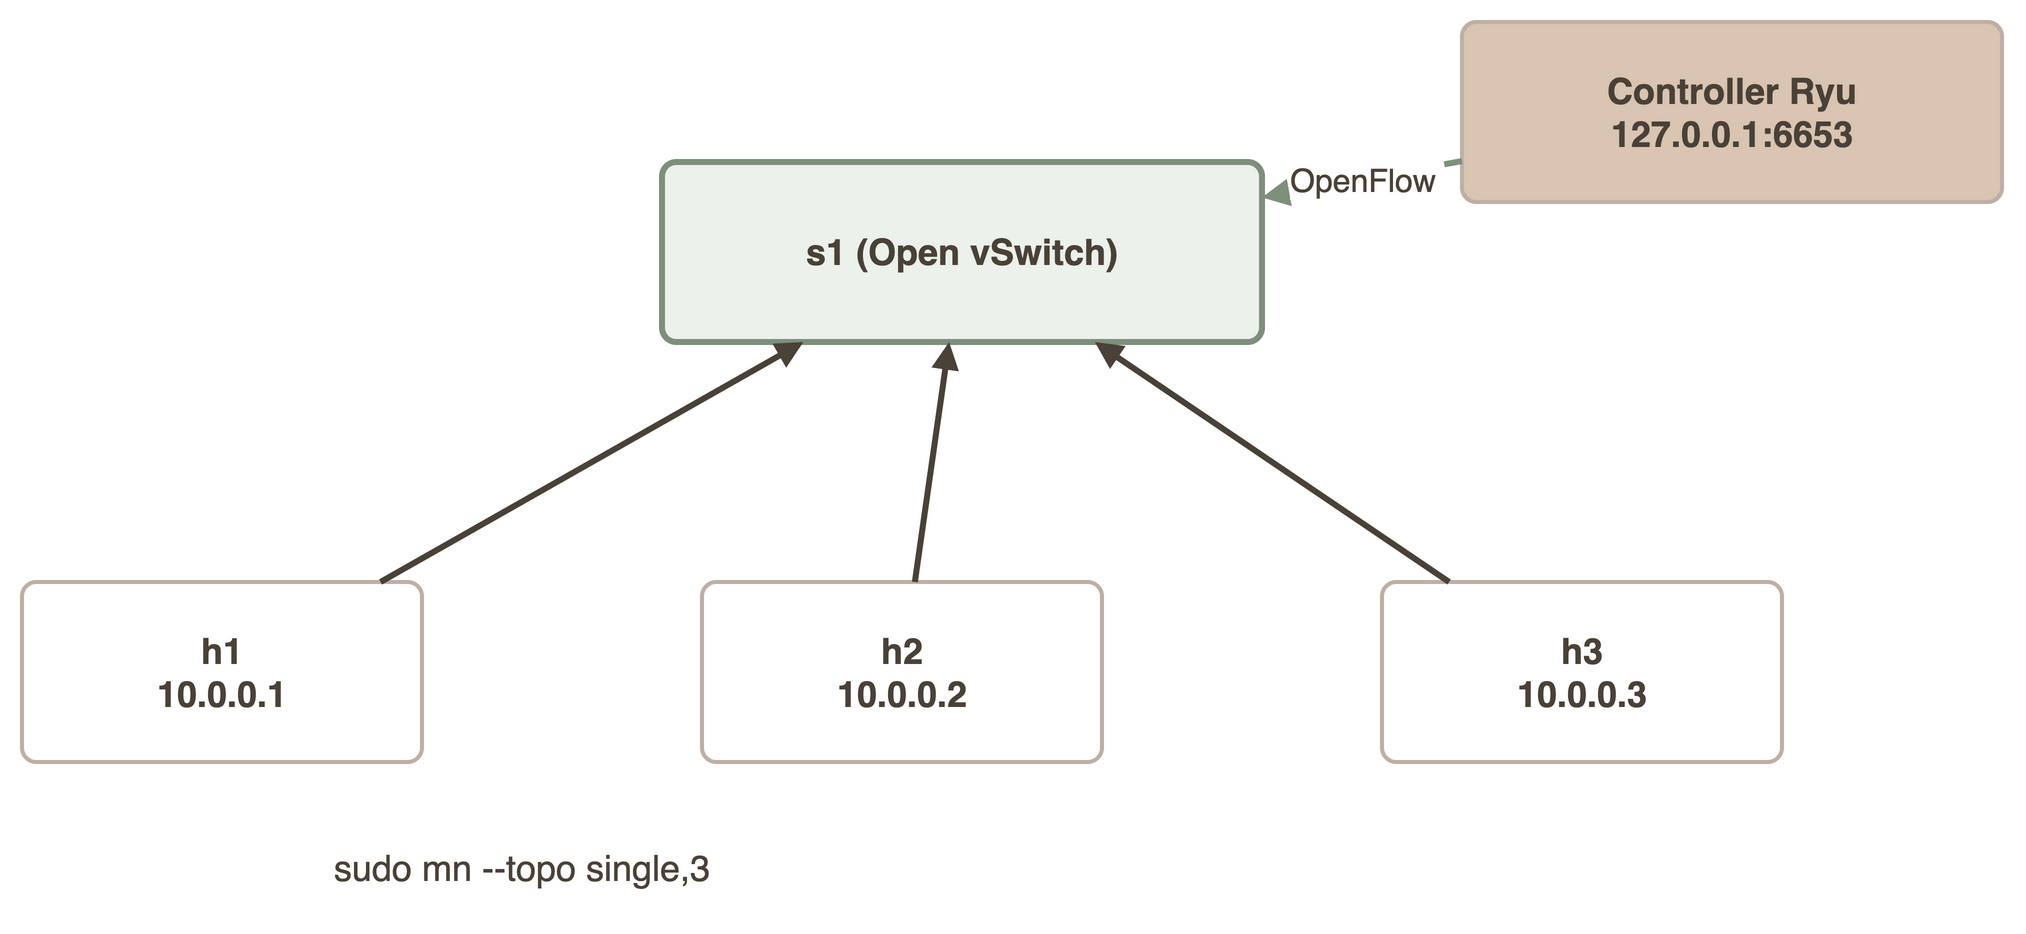
\includegraphics[width=\linewidth]{../Diagramas/g06-topologia.png}
\end{center}

\begin{leitura}
No centro está o switch \cmd{s1}, a verde. Os três hosts, \cmd{h1}, \cmd{h2} e \cmd{h3}, ligam-se a ele, cada um com o seu endereço IP. O controller, em cima à direita, liga-se ao switch por OpenFlow, representado a tracejado porque ainda não existe neste passo. A topologia é sempre a mesma ao longo do guião; o que muda é quem decide as regras do switch.
\end{leitura}

\begin{teoria}
Um switch OpenFlow não aprende endereços por si. Cada pacote é comparado com as entradas da tabela de fluxos e, se nenhuma corresponder, o resultado depende do \emph{fail-mode} do switch. No modo \emph{secure}, que o Mininet utiliza, o switch não encaminha o que não conhece. No modo \emph{standalone}, comportar-se-ia como um switch tradicional quando perdesse o controller.

A ação especial \cmd{NORMAL} pede ao switch que use a lógica clássica de camada 2: aprender endereços e inundar quando não conhece o destino. Instalar uma única regra com essa ação equivale a regressar ao switch tradicional, e é um exemplo extremo de modelo proativo: a regra foi instalada antes de haver tráfego, sem qualquer controller.

\textbf{A analisar neste passo:} a diferença entre ter um switch e ter um switch com regras. O hardware é o mesmo nas duas situações; o que muda é o conteúdo da tabela de fluxos.
\end{teoria}

\subsection*{2.1 Criação da topologia}

\begin{terminal}
sudo mn --topo single,3 --mac --switch ovsk,protocols=OpenFlow13 --controller none
\end{terminal}

\begin{saida}
*** Creating network
*** Adding controller
*** Adding hosts:
h1 h2 h3
*** Adding switches:
s1
*** Adding links:
(h1, s1) (h2, s1) (h3, s1)
*** Starting CLI:
mininet>
\end{saida}

O parâmetro \cmd{-{}-mac} atribui endereços MAC simples (\cmd{00:00:00:00:00:01}, \cmd{...:02}, \cmd{...:03}), mais fáceis de reconhecer. O parâmetro \cmd{protocols=OpenFlow13} fixa a versão do protocolo.

\subsection*{2.2 Teste de conectividade}

\begin{terminal}
mininet> pingall
\end{terminal}

\begin{saida}
*** Ping: testing ping reachability
h1 -> X X
h2 -> X X
h3 -> X X
*** Results: 100% dropped (0/6 received)
\end{saida}

\begin{observe}
Os três hosts estão ligados ao mesmo switch e nenhum alcança os outros. O que falta ao switch? Onde é que, nesta rede, estaria a informação necessária para decidir?
\end{observe}

\subsection*{2.3 A tabela de fluxos está vazia}

O comando \cmd{sh} da consola do Mininet executa um comando no sistema da máquina virtual.

\begin{terminal}
mininet> sh ovs-ofctl -O OpenFlow13 dump-flows s1
\end{terminal}

\begin{saida}
(sem entradas)
\end{saida}

\subsection*{2.4 Instalação de uma regra única}

\begin{terminal}
mininet> sh ovs-ofctl -O OpenFlow13 add-flow s1 actions=NORMAL
mininet> pingall
\end{terminal}

\begin{saida}
*** Ping: testing ping reachability
h1 -> h2 h3
h2 -> h1 h3
h3 -> h1 h2
*** Results: 0% dropped (6/6 received)
\end{saida}

\begin{erro}
\textbf{ovs-ofctl: s1 is not a bridge or a socket}: o Mininet não está a correr, ou o nome do switch está errado. Confirmar que o prompt \cmd{mininet>} está ativo e que o switch se chama \cmd{s1}.

\textbf{Os pings continuam a falhar após o add-flow}: confirmar com \cmd{dump-flows} que a regra foi instalada. Se a lista estiver vazia, repetir o comando e verificar a versão do protocolo (\cmd{-O OpenFlow13}).
\end{erro}

\begin{feito}
O \cmd{pingall} falhou sem regras e funcionou depois de instalada a regra \cmd{actions=NORMAL}.
\end{feito}

Sair do Mininet e limpar o ambiente antes do passo seguinte:

\begin{terminal}
mininet> exit
sudo mn -c
\end{terminal}

\passo{3}{Um controller reativo com o Ryu}

\textbf{Objetivo.} Escrever um controller que aprende a localização dos hosts, ligá-lo ao switch e observar a conectividade.

\textbf{Enquadramento.} Este passo concretiza o modelo reativo da Aula 06. O switch envia ao controller o primeiro pacote de cada fluxo, o controller decide e instala uma regra, e os pacotes seguintes já não passam por ele.

São necessários três terminais, todos ligados à mesma máquina virtual. Em cada novo terminal, executar \cmd{multipass shell icn-sdn}.

\begin{center}
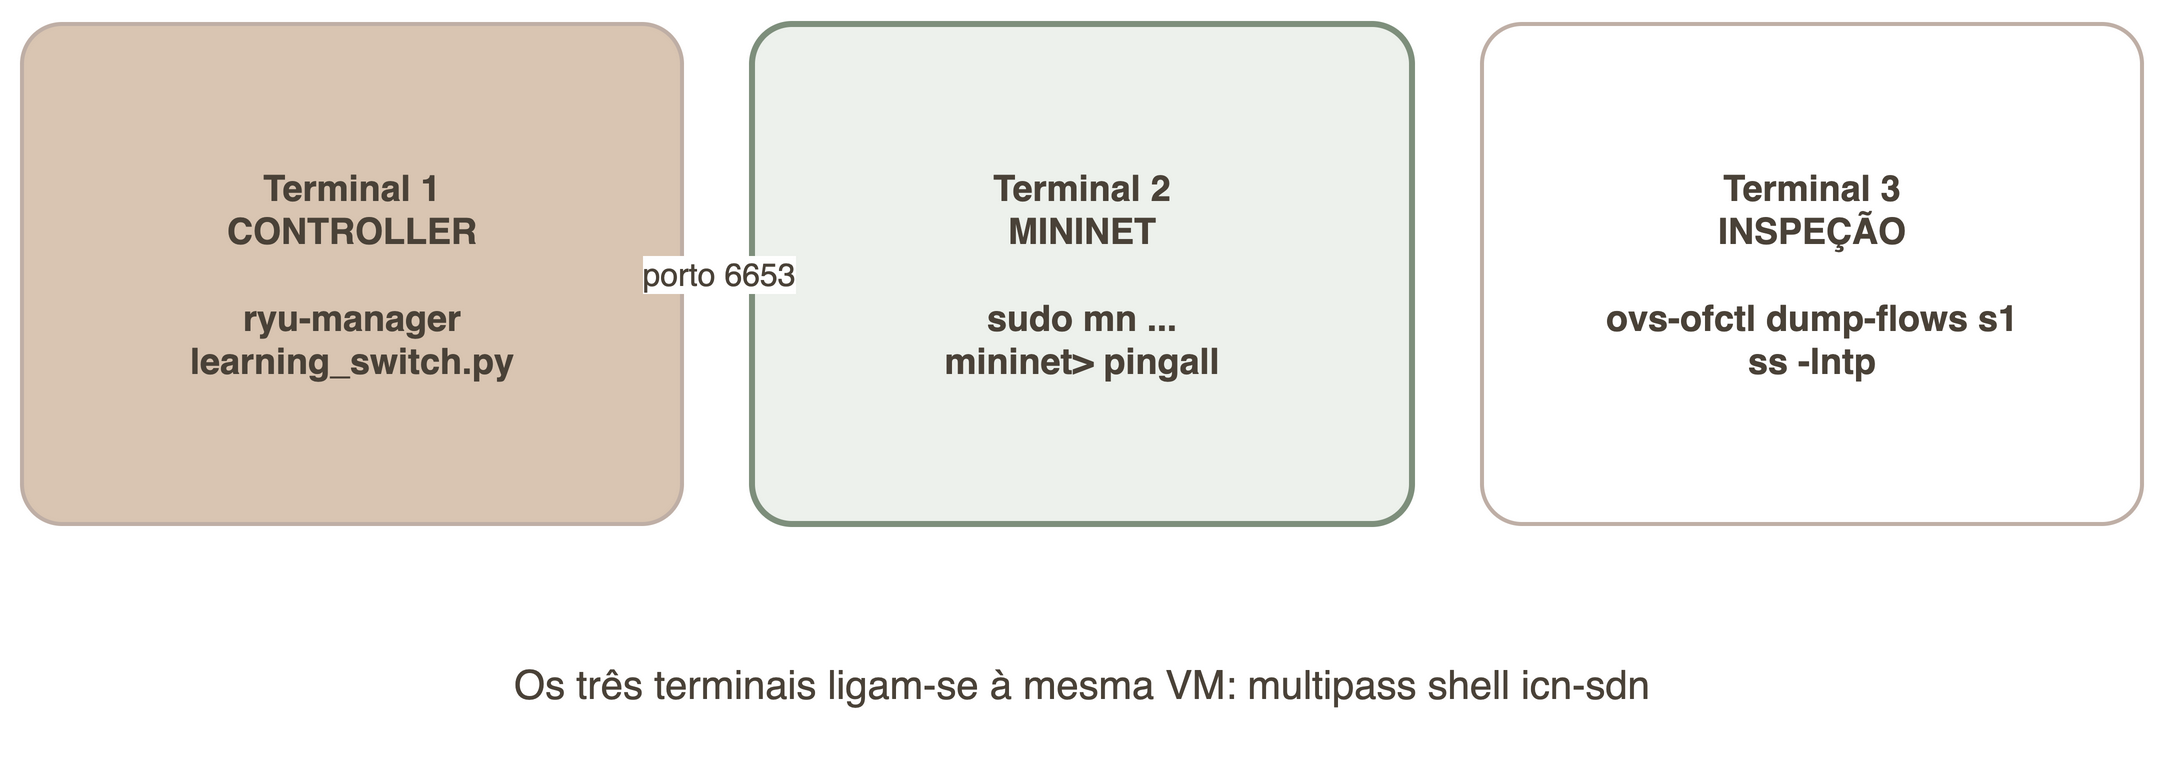
\includegraphics[width=\linewidth]{../Diagramas/g06-terminais.png}
\end{center}

\begin{leitura}
Cada caixa é um terminal. O terminal 1, a bege, executa o controller e deve ficar sempre aberto. O terminal 2, a verde, executa o Mininet, onde se escrevem os pings. O terminal 3, a branco, serve apenas para inspecionar: confirmar portos e listar fluxos sem interferir com os outros dois. A seta entre os dois primeiros indica que o Mininet se liga ao controller pelo porto 6653.
\end{leitura}

\begin{teoria}
Uma aplicação Ryu regista funções que reagem a eventos OpenFlow. O evento \cmd{EventOFPSwitchFeatures} ocorre quando um switch se liga, e é o momento de instalar a regra de último recurso: prioridade 0, qualquer pacote, enviar ao controller. É a entrada \emph{table-miss}. O evento \cmd{EventOFPPacketIn} ocorre sempre que o switch envia um pacote ao controller.

O \emph{learning switch} é a lógica clássica de camada 2, aqui em software. Ao receber um pacote, regista que o endereço MAC de origem está atrás da porta de entrada. Se já conhece a porta do destino, instala uma regra e encaminha. Se não conhece, inunda o pacote por todas as portas. É o mesmo algoritmo que um switch tradicional executa internamente, mas agora a correr fora do switch.

\textbf{A analisar neste passo:} onde está cada plano. O plano de controlo é o ficheiro Python, e o plano de dados é a tabela de fluxos do Open vSwitch.
\end{teoria}

\subsection*{3.1 Ficheiro do controller}

No terminal 1, criar o ficheiro \cmd{learning\_switch.py} na pasta \cmd{icn-aula06} com o conteúdo seguinte, utilizando o \cmd{nano} (\cmd{nano \textasciitilde/icn-aula06/learning\_switch.py}).

\begin{ficheiro}{learning\_switch.py}
from ryu.base import app_manager
from ryu.controller import ofp_event
from ryu.controller.handler import CONFIG_DISPATCHER, MAIN_DISPATCHER, set_ev_cls
from ryu.ofproto import ofproto_v1_3
from ryu.lib.packet import packet, ethernet


class LearningSwitch(app_manager.RyuApp):
    OFP_VERSIONS = [ofproto_v1_3.OFP_VERSION]

    def __init__(self, *args, **kwargs):
        super().__init__(*args, **kwargs)
        self.mac_to_port = {}

    @set_ev_cls(ofp_event.EventOFPSwitchFeatures, CONFIG_DISPATCHER)
    def switch_features(self, ev):
        dp = ev.msg.datapath
        ofp, parser = dp.ofproto, dp.ofproto_parser
        actions = [parser.OFPActionOutput(ofp.OFPP_CONTROLLER, ofp.OFPCML_NO_BUFFER)]
        self.add_flow(dp, 0, parser.OFPMatch(), actions)

    def add_flow(self, dp, priority, match, actions, idle=0):
        ofp, parser = dp.ofproto, dp.ofproto_parser
        inst = [parser.OFPInstructionActions(ofp.OFPIT_APPLY_ACTIONS, actions)]
        dp.send_msg(parser.OFPFlowMod(datapath=dp, priority=priority, match=match,
                                      instructions=inst, idle_timeout=idle))

    @set_ev_cls(ofp_event.EventOFPPacketIn, MAIN_DISPATCHER)
    def packet_in(self, ev):
        msg = ev.msg
        dp = msg.datapath
        ofp, parser = dp.ofproto, dp.ofproto_parser
        in_port = msg.match["in_port"]
        eth = packet.Packet(msg.data).get_protocols(ethernet.ethernet)[0]

        table = self.mac_to_port.setdefault(dp.id, {})
        table[eth.src] = in_port
        out_port = table.get(eth.dst, ofp.OFPP_FLOOD)
        actions = [parser.OFPActionOutput(out_port)]

        if out_port != ofp.OFPP_FLOOD:
            match = parser.OFPMatch(in_port=in_port, eth_dst=eth.dst)
            self.add_flow(dp, 1, match, actions, idle=60)

        data = msg.data if msg.buffer_id == ofp.OFP_NO_BUFFER else None
        dp.send_msg(parser.OFPPacketOut(datapath=dp, buffer_id=msg.buffer_id,
                                        in_port=in_port, actions=actions, data=data))
\end{ficheiro}

\begin{erro}
O Python distingue maiúsculas de minúsculas e depende da indentação, feita com espaços. Se o ficheiro for gravado com tabulações, o Ryu indica \cmd{IndentationError}. Rever o ficheiro e substituir as tabulações por quatro espaços.
\end{erro}

\subsection*{3.2 Arranque do controller}

Ainda no terminal 1:

\begin{terminal}
~/ryu-env/bin/ryu-manager ~/icn-aula06/learning_switch.py
\end{terminal}

\begin{saida}
loading app /home/ubuntu/icn-aula06/learning_switch.py
loading app ryu.controller.ofp_handler
instantiating app /home/ubuntu/icn-aula06/learning_switch.py of LearningSwitch
instantiating app ryu.controller.ofp_handler of OFPHandler
\end{saida}

O terminal fica ocupado: é o comportamento esperado. Deve permanecer aberto até ao fim do passo 5.

\subsection*{3.3 Confirmação do porto}

No terminal 3, confirmar que o controller está à escuta:

\begin{terminal}
sudo ss -lntp | grep 6653
\end{terminal}

\begin{saida}
LISTEN 0  128  0.0.0.0:6653  0.0.0.0:*  users:(("ryu-manager",pid=3120,fd=6))
\end{saida}

\begin{erro}
Se não aparecer nenhuma linha, o controller não está a correr, ou usa outro porto. Confirmar o terminal 1. Se o porto indicado for o 6633, que é o valor histórico, usar esse valor no comando seguinte.
\end{erro}

\subsection*{3.4 Ligação do Mininet ao controller}

No terminal 2:

\begin{terminal}
sudo mn --topo single,3 --mac --switch ovsk,protocols=OpenFlow13 \
  --controller remote,ip=127.0.0.1,port=6653
\end{terminal}

\begin{terminal}
mininet> pingall
\end{terminal}

\begin{saida}
*** Ping: testing ping reachability
h1 -> h2 h3
h2 -> h1 h3
h3 -> h1 h2
*** Results: 0% dropped (6/6 received)
\end{saida}

Para confirmar que o switch está efetivamente ligado ao controller, no terminal 3:

\begin{terminal}
sudo ovs-vsctl show
\end{terminal}

\begin{saida}
    Bridge s1
        Controller "tcp:127.0.0.1:6653"
            is_connected: true
        fail_mode: secure
        Port s1-eth1
        Port s1-eth2
        Port s1-eth3
\end{saida}

\begin{observe}
O resultado é o do passo 2 com a regra \cmd{NORMAL}, mas a origem é diferente. Desta vez, quem tomou as decisões foi um programa em Python que se pode ler e modificar. Onde está a linha \cmd{is\_connected: true} e o que significaria \cmd{false}?
\end{observe}

\begin{erro}
\textbf{O pingall falha com o controller a correr}: confirmar \cmd{is\_connected: true} com \cmd{ovs-vsctl show}. Se for \cmd{false}, o porto do comando está errado ou o controller não arrancou. Sair do Mininet, executar \cmd{sudo mn -c} e repetir com o porto confirmado em 3.3.
\end{erro}

\begin{feito}
O \cmd{pingall} apresenta \cmd{0\% dropped} e o \cmd{ovs-vsctl show} indica \cmd{is\_connected: true}.
\end{feito}

\passo{4}{A tabela de fluxos}

\textbf{Objetivo.} Ler a tabela de fluxos construída pelo controller, identificar prioridade, contadores e \emph{timeouts}, e observar a reconstrução reativa de uma regra.

\textbf{Enquadramento.} A tabela de fluxos é o ponto de contacto entre o plano de controlo e o plano de dados. Tudo o que o controller decidiu fica ali registado, com números que permitem verificar o que realmente aconteceu.

\begin{center}
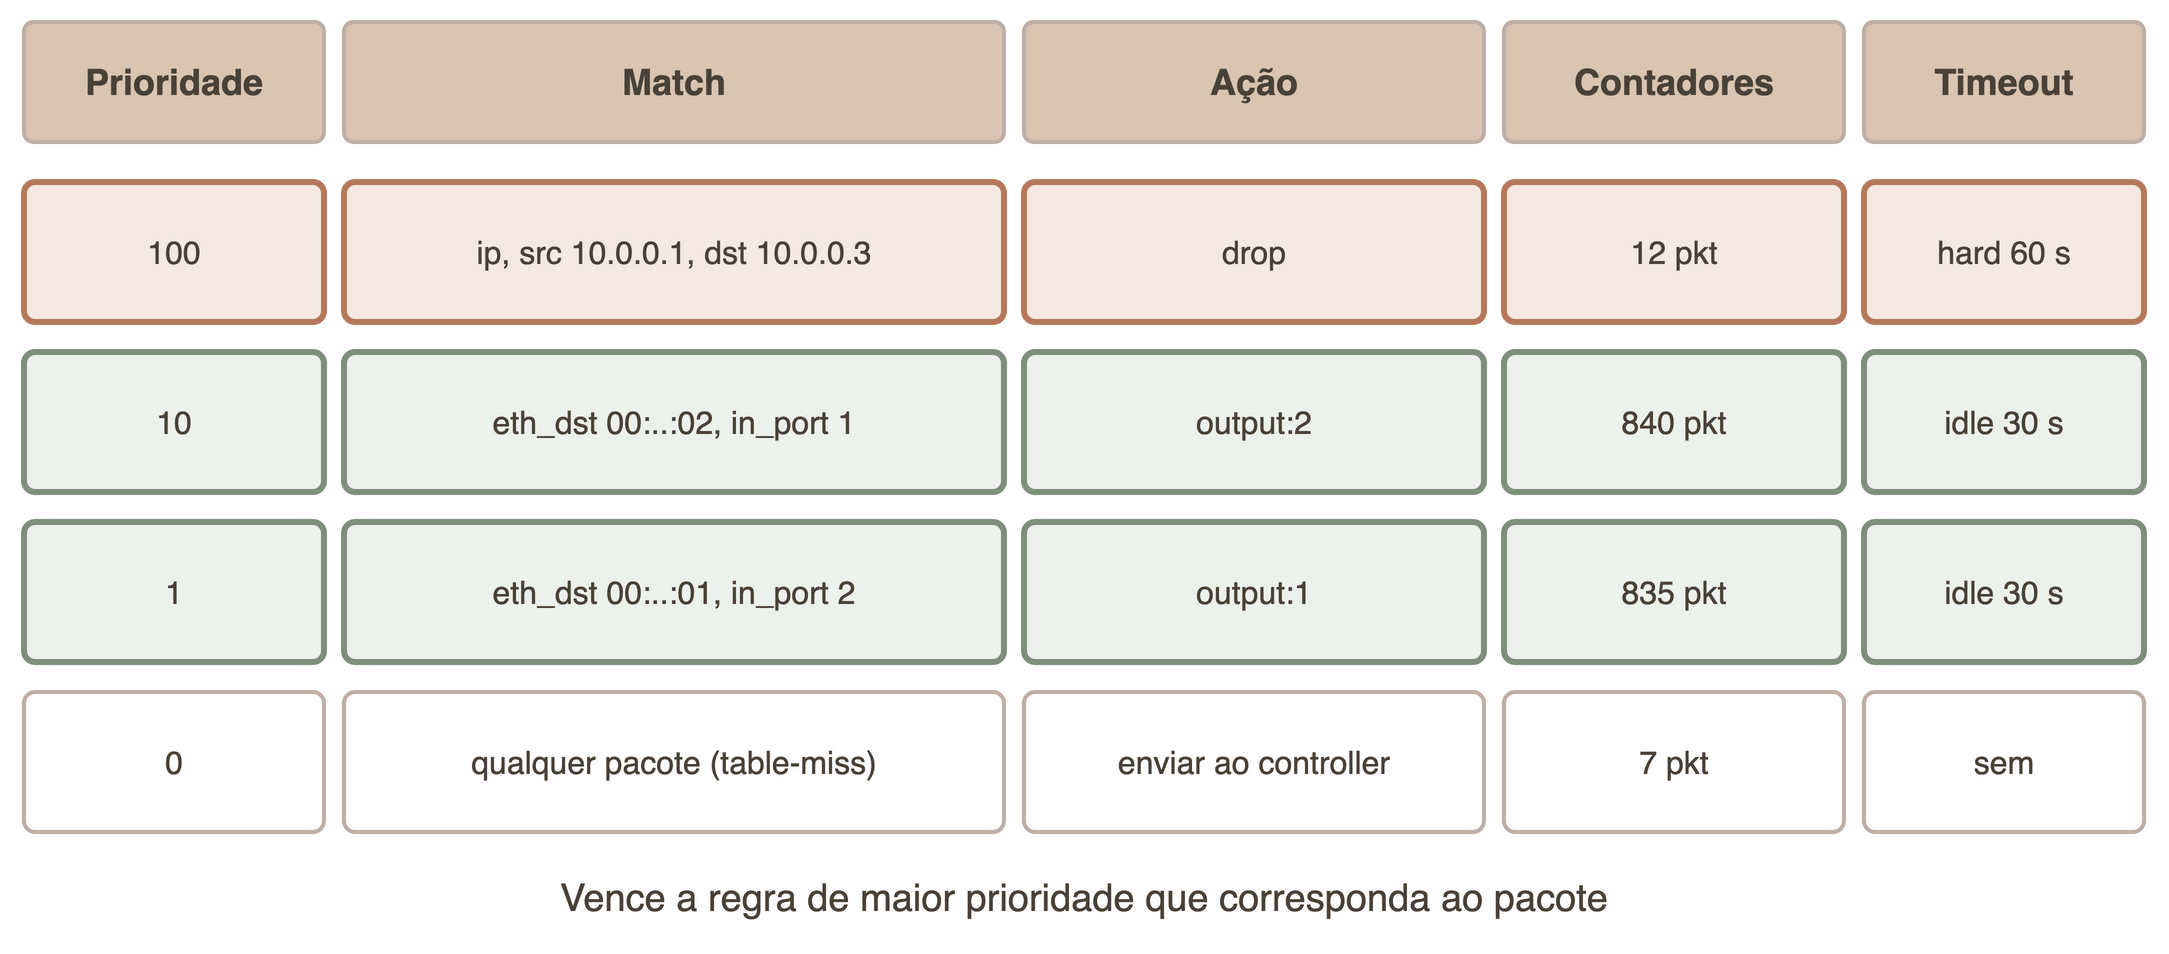
\includegraphics[width=\linewidth]{../Diagramas/a06-tabela-fluxos.png}
\end{center}

\begin{leitura}
A figura é a mesma tabela de fluxos apresentada na aula. As colunas são as grandezas que se vão procurar no resultado de \cmd{dump-flows}: a prioridade, o \emph{match}, a ação, os contadores e os \emph{timeouts}. A linha de baixo, de prioridade 0, é a entrada \emph{table-miss} que o controller instalou quando o switch se ligou. As restantes foram criadas à medida que o tráfego foi chegando.
\end{leitura}

\begin{teoria}
Cada entrada da tabela guarda os contadores \cmd{n\_packets} e \cmd{n\_bytes}, que o switch incrementa a cada pacote que corresponde. Não é necessário nenhum software adicional para medir o tráfego por fluxo. O campo \cmd{idle\_timeout} indica ao switch que remova a entrada depois de um período sem pacotes, e o campo \cmd{duration} mostra há quanto tempo a entrada existe.

Quando uma entrada é removida, ou apagada à mão, o próximo pacote do fluxo volta a não encontrar regra e regressa ao controller. O mecanismo reativo repete-se: o controller decide de novo e reinstala a regra. É por isso que o primeiro \cmd{ping} depois de uma remoção demora mais do que os seguintes.

\textbf{A analisar neste passo:} a relação entre o que se vê na tabela e o tráfego que se gerou. Cada contador responde à pergunta: quantos pacotes usaram esta regra?
\end{teoria}

\subsection*{4.1 Leitura da tabela}

No terminal 3:

\begin{terminal}
sudo ovs-ofctl -O OpenFlow13 dump-flows s1
\end{terminal}

\begin{saida}
 cookie=0x0, duration=95.2s, table=0, n_packets=6, n_bytes=468, idle_timeout=60, priority=1,in_port="s1-eth1",dl_dst=00:00:00:00:00:02 actions=output:"s1-eth2"
 cookie=0x0, duration=95.2s, table=0, n_packets=6, n_bytes=468, idle_timeout=60, priority=1,in_port="s1-eth2",dl_dst=00:00:00:00:00:01 actions=output:"s1-eth1"
 cookie=0x0, duration=103.9s, table=0, n_packets=18, n_bytes=1436, priority=0 actions=CONTROLLER:65535
\end{saida}

Os nomes e os valores dependem do tráfego já gerado. Procurar nas entradas os campos \cmd{priority}, \cmd{n\_packets}, \cmd{idle\_timeout} e \cmd{duration}.

\subsection*{4.2 Os contadores aumentam}

No terminal 2:

\begin{terminal}
mininet> h1 ping -c 5 h2
\end{terminal}

Voltar ao terminal 3 e repetir o \cmd{dump-flows}. O valor de \cmd{n\_packets} das duas primeiras entradas deve ter aumentado em 5, uma por cada pedido e resposta.

\subsection*{4.3 Remoção das regras}

\begin{terminal}
mininet> sh ovs-ofctl -O OpenFlow13 del-flows s1
mininet> sh ovs-ofctl -O OpenFlow13 dump-flows s1
\end{terminal}

\begin{saida}
(sem entradas)
\end{saida}

A remoção apagou também a entrada \emph{table-miss}. Para que o switch volte a consultar o controller, é necessário reiniciar a ligação:

\begin{terminal}
mininet> sh ovs-vsctl del-controller s1
mininet> sh ovs-vsctl set-controller s1 tcp:127.0.0.1:6653
mininet> h1 ping -c 3 h2
\end{terminal}

\begin{saida}
64 bytes from 10.0.0.2: icmp_seq=1 ttl=64 time=21.3 ms
64 bytes from 10.0.0.2: icmp_seq=2 ttl=64 time=0.112 ms
64 bytes from 10.0.0.2: icmp_seq=3 ttl=64 time=0.067 ms
\end{saida}

\begin{observe}
O primeiro pacote demorou muito mais do que os seguintes. Que percurso fez? Que mensagens trocaram o switch e o controller antes de ele ser entregue?
\end{observe}

\begin{erro}
\textbf{ping: connect: Network is unreachable} ou \cmd{100\% packet loss} depois da remoção: o switch ficou sem a entrada \emph{table-miss} e sem controller. Repetir os dois comandos \cmd{ovs-vsctl} desta secção.
\end{erro}

\subsection*{4.4 Expiração por inatividade}

Aguardar mais de 60 segundos sem gerar tráfego e listar de novo a tabela:

\begin{terminal}
sudo ovs-ofctl -O OpenFlow13 dump-flows s1
\end{terminal}

As entradas com \cmd{idle\_timeout=60} desaparecem, e a entrada \emph{table-miss} permanece, porque foi instalada sem \emph{timeout}.

\begin{feito}
Foi lida a tabela de fluxos, observado o aumento dos contadores, e verificado que a remoção de uma regra obriga o primeiro pacote a voltar ao controller.
\end{feito}

\passo{5}{Uma política de bloqueio}

\textbf{Objetivo.} Bloquear o tráfego entre \cmd{h1} e \cmd{h3}, mantendo a comunicação com \cmd{h2}, e observar o efeito da prioridade e do \emph{timeout}.

\textbf{Enquadramento.} Uma política de rede traduz-se em regras com \emph{match} mais específico e prioridade superior à das regras genéricas. É o mecanismo que, em ponto pequeno, sustenta a microssegmentação apresentada na aula.

\begin{center}
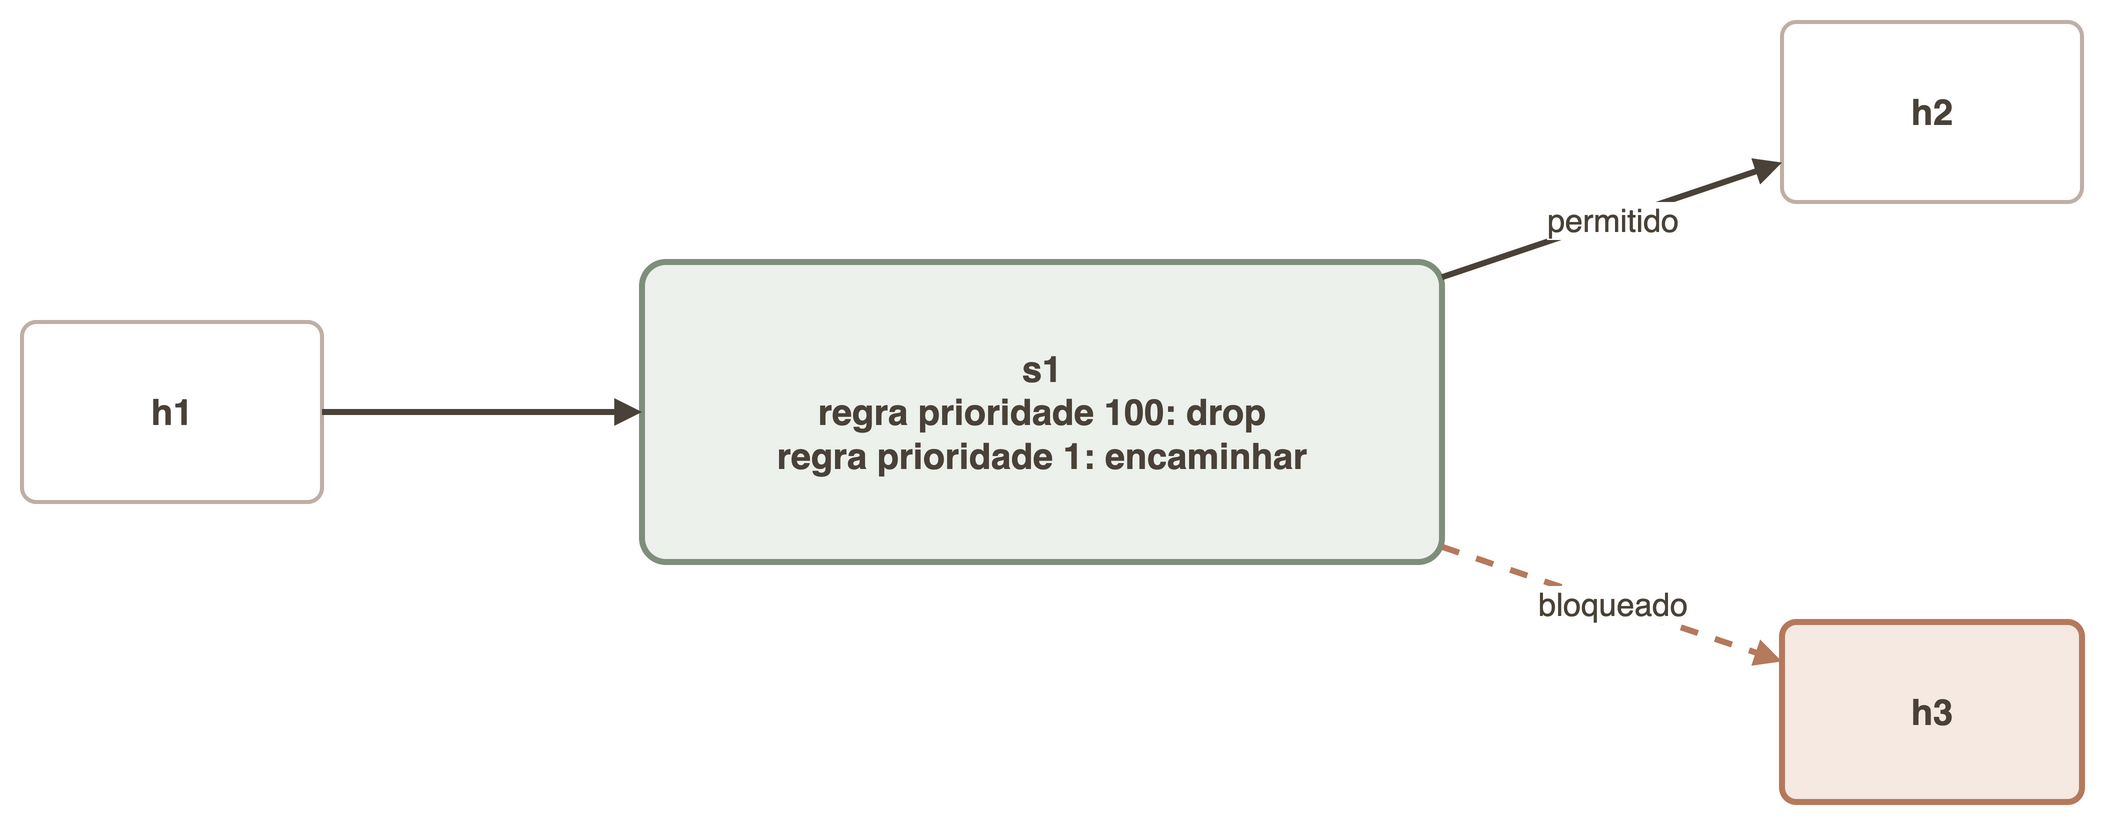
\includegraphics[width=\linewidth]{../Diagramas/g06-politica.png}
\end{center}

\begin{leitura}
O host \cmd{h1} envia tráfego para o switch. No switch coexistem duas regras que podem corresponder ao mesmo pacote: a de prioridade 100, que descarta o tráfego de \cmd{h1} para \cmd{h3}, e a de prioridade 1, que encaminha o tráfego em geral. A seta para \cmd{h2}, a cheio, representa o tráfego permitido. A seta para \cmd{h3}, a tracejado e a vermelho, representa o tráfego que a regra de maior prioridade descarta.
\end{leitura}

\begin{teoria}
Quando duas regras correspondem ao mesmo pacote, o switch aplica a de maior prioridade. A regra de encaminhamento do controller tem prioridade 1, pelo que uma regra de bloqueio com prioridade 100 prevalece sem ser necessário alterar o controller. A ação \cmd{drop} não é uma instrução: é a ausência de ações. Uma entrada sem ações descarta os pacotes que correspondem.

O \emph{match} desta regra usa campos de camada 3, \cmd{ip}, \cmd{nw\_src} e \cmd{nw\_dst}, enquanto as regras do controller usam apenas camada 2. A regra não bloqueia os pedidos ARP, porque estes não são pacotes IP. O \cmd{h1} consegue descobrir o endereço MAC do \cmd{h3}, mas os pacotes IP seguintes são descartados.

O \cmd{hard\_timeout} remove a regra ao fim de um tempo fixo, independentemente do tráfego. Neste exercício serve para demonstrar uma política temporária que se levanta sozinha.

\textbf{A analisar neste passo:} a ordem de aplicação, que depende da prioridade e não da ordem de instalação das regras.
\end{teoria}

\subsection*{5.1 Instalação da regra}

No terminal 2, com o Mininet ainda em execução:

\begin{terminal}
mininet> sh ovs-ofctl -O OpenFlow13 add-flow s1 "hard_timeout=60,priority=100,ip,nw_src=10.0.0.1,nw_dst=10.0.0.3,actions=drop"
\end{terminal}

\subsection*{5.2 Verificação}

\begin{terminal}
mininet> h1 ping -c 3 h3
mininet> h1 ping -c 3 h2
\end{terminal}

\begin{saida}
3 packets transmitted, 0 received, 100% packet loss, time 2049ms
3 packets transmitted, 3 received, 0% packet loss, time 2003ms
\end{saida}

\begin{terminal}
mininet> sh ovs-ofctl -O OpenFlow13 dump-flows s1
\end{terminal}

\begin{saida}
 cookie=0x0, duration=14.2s, table=0, n_packets=3, n_bytes=294, hard_timeout=60, priority=100,ip,nw_src=10.0.0.1,nw_dst=10.0.0.3 actions=drop
 ...
\end{saida}

O contador \cmd{n\_packets} da regra de bloqueio indica quantos pacotes foram descartados.

\subsection*{5.3 Expiração da política}

Aguardar 60 segundos desde a instalação e repetir:

\begin{terminal}
mininet> h1 ping -c 3 h3
\end{terminal}

\begin{saida}
3 packets transmitted, 3 received, 0% packet loss, time 2003ms
\end{saida}

\begin{observe}
Quem aplicou a política, o controller ou o switch? Em que local ficou escrita, e o que mudaria se o controller fosse reiniciado enquanto a regra existia?
\end{observe}

\begin{erro}
\textbf{O ping para h3 continua a funcionar}: o \cmd{hard\_timeout} pode já ter terminado, ou a regra não foi instalada. Confirmar com \cmd{dump-flows} e repetir o \cmd{add-flow}.
\end{erro}

\begin{feito}
O tráfego \cmd{h1} para \cmd{h3} foi descartado e o tráfego \cmd{h1} para \cmd{h2} manteve-se, e a política expirou ao fim de 60 segundos.
\end{feito}

\section*{Desafio opcional: a política no controller}

Mover a política para o plano de controlo. Em vez de instalar a regra com o \cmd{ovs-ofctl}, modificar o ficheiro \cmd{learning\_switch.py}: no método \cmd{packet\_in}, antes de calcular \cmd{out\_port}, acrescentar uma verificação dos endereços MAC.

\begin{ficheiro}{learning\_switch.py (acrescento)}
BLOQUEADOS = {("00:00:00:00:00:01", "00:00:00:00:00:03"),
              ("00:00:00:00:00:03", "00:00:00:00:00:01")}

# dentro de packet_in, antes de calcular out_port:
if (eth.src, eth.dst) in BLOQUEADOS:
    match = parser.OFPMatch(in_port=in_port, eth_src=eth.src, eth_dst=eth.dst)
    self.add_flow(dp, 100, match, [], idle=60)
    return
\end{ficheiro}

Parar o controller no terminal 1 com \cmd{Ctrl+C}, repetir o passo 3.2, sair do Mininet com \cmd{exit}, executar \cmd{sudo mn -c} e repetir o passo 3.4. Verificar com \cmd{h1 ping -c 3 h3} e \cmd{h1 ping -c 3 h2}.

\begin{observe}
Qual a vantagem de a política viver no controller, em vez de ser instalada à mão em cada switch? E se a rede tivesse cinquenta switches?
\end{observe}

\passo{6}{Um túnel VXLAN}

\textbf{Objetivo.} Criar uma rede overlay entre dois namespaces, sobre uma rede subjacente, e observar o encapsulamento VXLAN em UDP.

\textbf{Enquadramento.} Os Pods do Kubernetes e as máquinas virtuais do Proxmox comunicam através de túneis como este. A diferença é que aqui o túnel é criado à mão, passo a passo, o que torna visível cada parte.

Este passo é independente do Mininet. Pode ser feito no terminal 3, ou em qualquer terminal da máquina virtual, depois de sair do Mininet com \cmd{exit} e de executar \cmd{sudo mn -c}.

\begin{center}
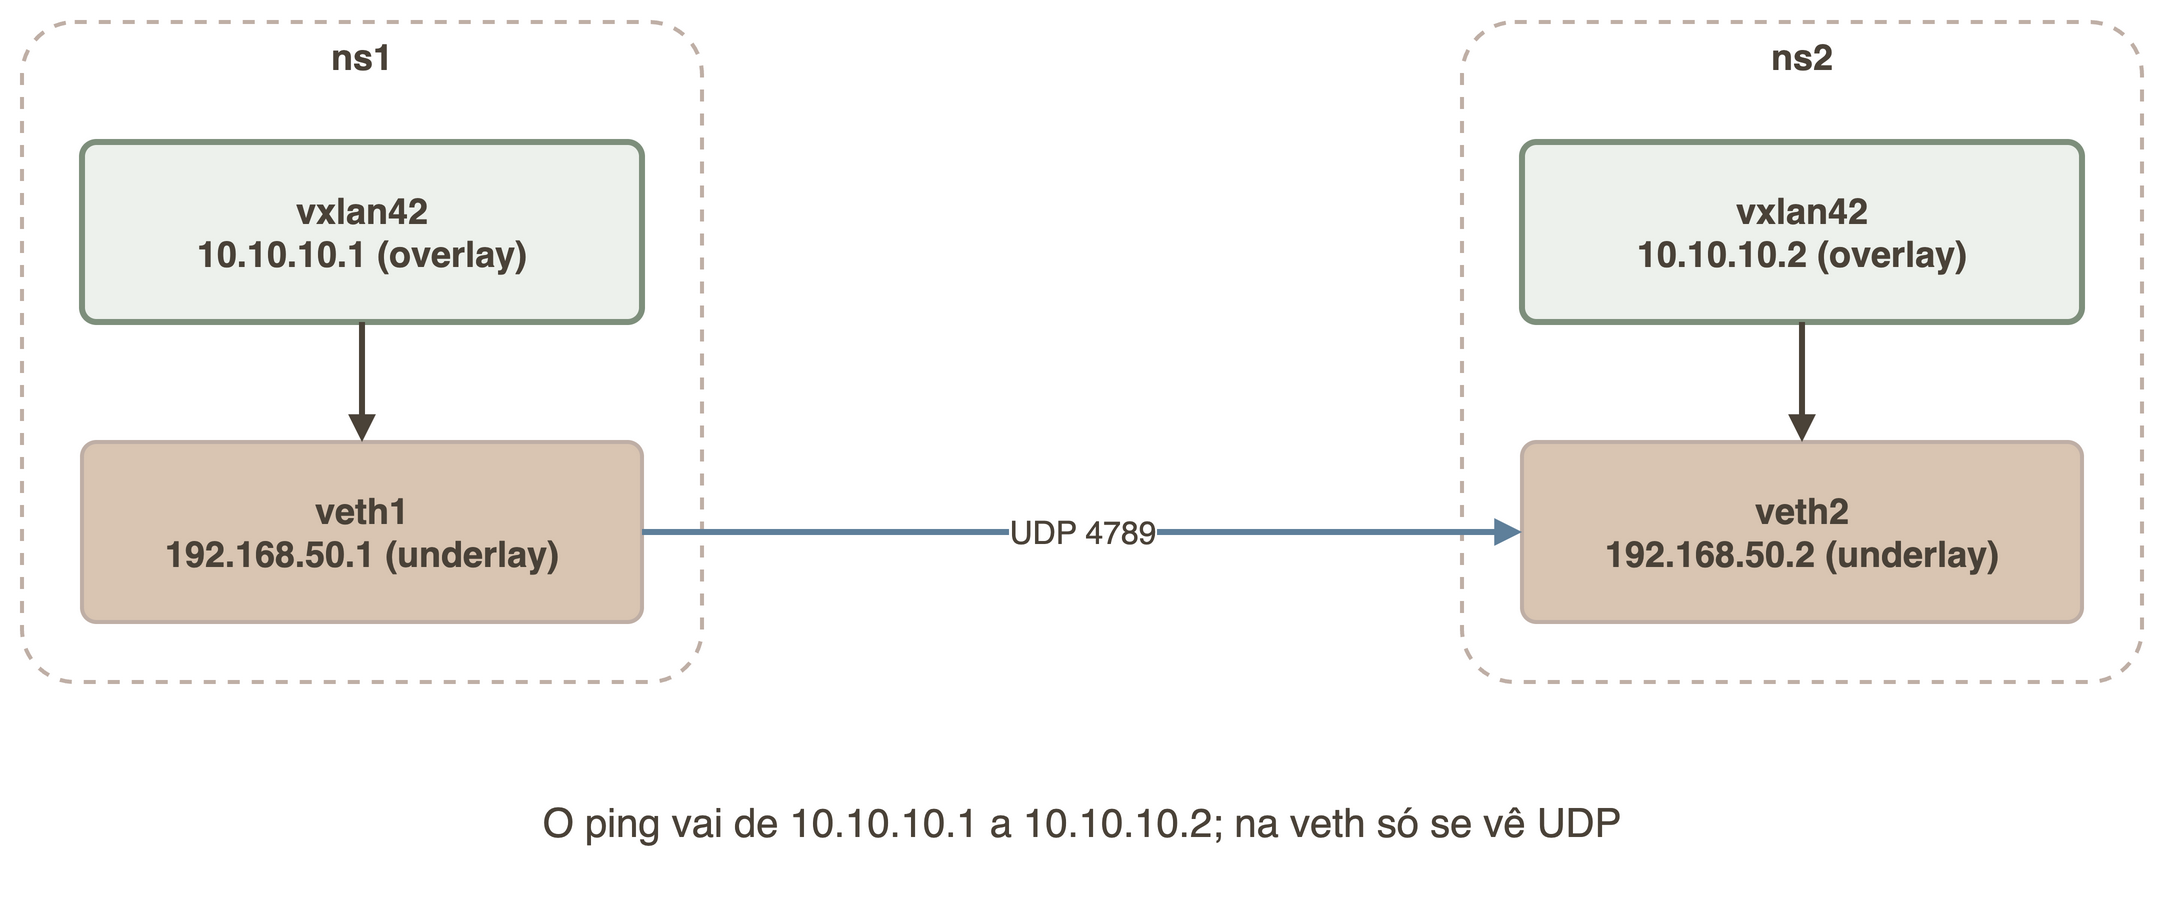
\includegraphics[width=\linewidth]{../Diagramas/g06-vxlan-ns.png}
\end{center}

\begin{leitura}
Cada caixa tracejada é um namespace de rede, \cmd{ns1} à esquerda e \cmd{ns2} à direita. Em baixo, a bege, está o \emph{underlay}: um par de interfaces \cmd{veth} com endereços da rede 192.168.50.0/24, ligadas entre si. Em cima, a verde, está o \emph{overlay}: as interfaces \cmd{vxlan42}, com endereços da rede 10.10.10.0/24. Os pacotes do overlay descem para o underlay, atravessam-no em UDP no porto 4789 e voltam a subir no outro lado.
\end{leitura}

\begin{teoria}
Um namespace de rede é uma pilha de rede isolada, com as suas interfaces, tabelas de rotas e regras de firewall. É o mesmo mecanismo de isolamento dos containers da Aula 04. Um par \emph{veth} é um cabo virtual: o que entra numa ponta sai na outra.

Uma interface VXLAN tem um identificador de rede, o VNI, e um destino remoto. Os pacotes que lhe são entregues são embrulhados em UDP e enviados ao destino remoto pela interface subjacente. O \cmd{ip} do Linux executa as funções de VTEP. O identificador 42 é arbitrário, mas tem de ser o mesmo nas duas extremidades.

O cabeçalho adicional ocupa 50 bytes. O Linux ajusta o MTU da interface overlay para 1450, de modo que um pacote encapsulado caiba no MTU de 1500 do underlay.

\textbf{A analisar neste passo:} a diferença entre o que os dois namespaces veem, pacotes IP normais entre 10.10.10.1 e 10.10.10.2, e o que passa na rede subjacente, UDP entre 192.168.50.1 e 192.168.50.2.
\end{teoria}

\subsection*{6.1 Criação do underlay}

\begin{terminal}
sudo ip netns add ns1
sudo ip netns add ns2
sudo ip link add veth1 type veth peer name veth2
sudo ip link set veth1 netns ns1
sudo ip link set veth2 netns ns2
sudo ip netns exec ns1 ip addr add 192.168.50.1/24 dev veth1
sudo ip netns exec ns2 ip addr add 192.168.50.2/24 dev veth2
sudo ip netns exec ns1 ip link set veth1 up
sudo ip netns exec ns2 ip link set veth2 up
sudo ip netns exec ns1 ping -c 2 192.168.50.2
\end{terminal}

\begin{saida}
64 bytes from 192.168.50.2: icmp_seq=1 ttl=64 time=0.071 ms
64 bytes from 192.168.50.2: icmp_seq=2 ttl=64 time=0.048 ms
\end{saida}

\subsection*{6.2 Criação do overlay}

\begin{terminal}
sudo ip netns exec ns1 ip link add vxlan42 type vxlan id 42 dev veth1 remote 192.168.50.2 dstport 4789
sudo ip netns exec ns2 ip link add vxlan42 type vxlan id 42 dev veth2 remote 192.168.50.1 dstport 4789
sudo ip netns exec ns1 ip addr add 10.10.10.1/24 dev vxlan42
sudo ip netns exec ns2 ip addr add 10.10.10.2/24 dev vxlan42
sudo ip netns exec ns1 ip link set vxlan42 up
sudo ip netns exec ns2 ip link set vxlan42 up
sudo ip netns exec ns1 ip -d link show vxlan42
\end{terminal}

\begin{saida}
vxlan42: <BROADCAST,MULTICAST,UP,LOWER_UP> mtu 1450 ...
    vxlan id 42 remote 192.168.50.2 dev veth1 srcport 0 0 dstport 4789 ...
\end{saida}

\subsection*{6.3 Teste e captura}

Abrir um segundo terminal da máquina virtual e iniciar a captura no underlay:

\begin{terminal}
sudo ip netns exec ns1 tcpdump -ni veth1 -c 4 udp port 4789
\end{terminal}

No primeiro terminal, gerar tráfego no overlay:

\begin{terminal}
sudo ip netns exec ns1 ping -c 2 10.10.10.2
\end{terminal}

\begin{saida}
IP 192.168.50.1.43512 > 192.168.50.2.4789: VXLAN, flags [I] (0x08), vni 42
IP 10.10.10.1 > 10.10.10.2: ICMP echo request, id 11, seq 1, length 64
IP 192.168.50.2.43512 > 192.168.50.1.4789: VXLAN, flags [I] (0x08), vni 42
IP 10.10.10.2 > 10.10.10.1: ICMP echo reply, id 11, seq 1, length 64
\end{saida}

\begin{observe}
Cada pacote aparece em duas camadas: um IP externo, entre os endereços do underlay, e um IP interno, entre os endereços do overlay. Qual dos dois é visível para a rede física? E o que seria necessário alterar na rede física para criar uma segunda rede overlay com o VNI 43?
\end{observe}

\begin{erro}
\textbf{Cannot find device veth1} ou \cmd{RTNETLINK answers: File exists}: um passo anterior falhou ou foi repetido. Executar \cmd{sudo ip netns del ns1}, \cmd{sudo ip netns del ns2} e recomeçar em 6.1.

\textbf{tcpdump: command not found}: instalar com \cmd{sudo apt install -y tcpdump}.

\textbf{O ping no overlay falha}: confirmar com \cmd{ip -d link show vxlan42} que os dois lados têm o mesmo VNI e que os endereços remotos estão trocados.
\end{erro}

\begin{feito}
O \cmd{tcpdump} mostra pacotes UDP no porto 4789 com \cmd{vni 42} a transportar os pedidos e respostas ICMP do overlay.
\end{feito}

\passo{7}{Limpeza}

\textbf{Objetivo.} Terminar o controller, apagar a topologia e a máquina virtual, libertando todos os recursos.

\begin{center}
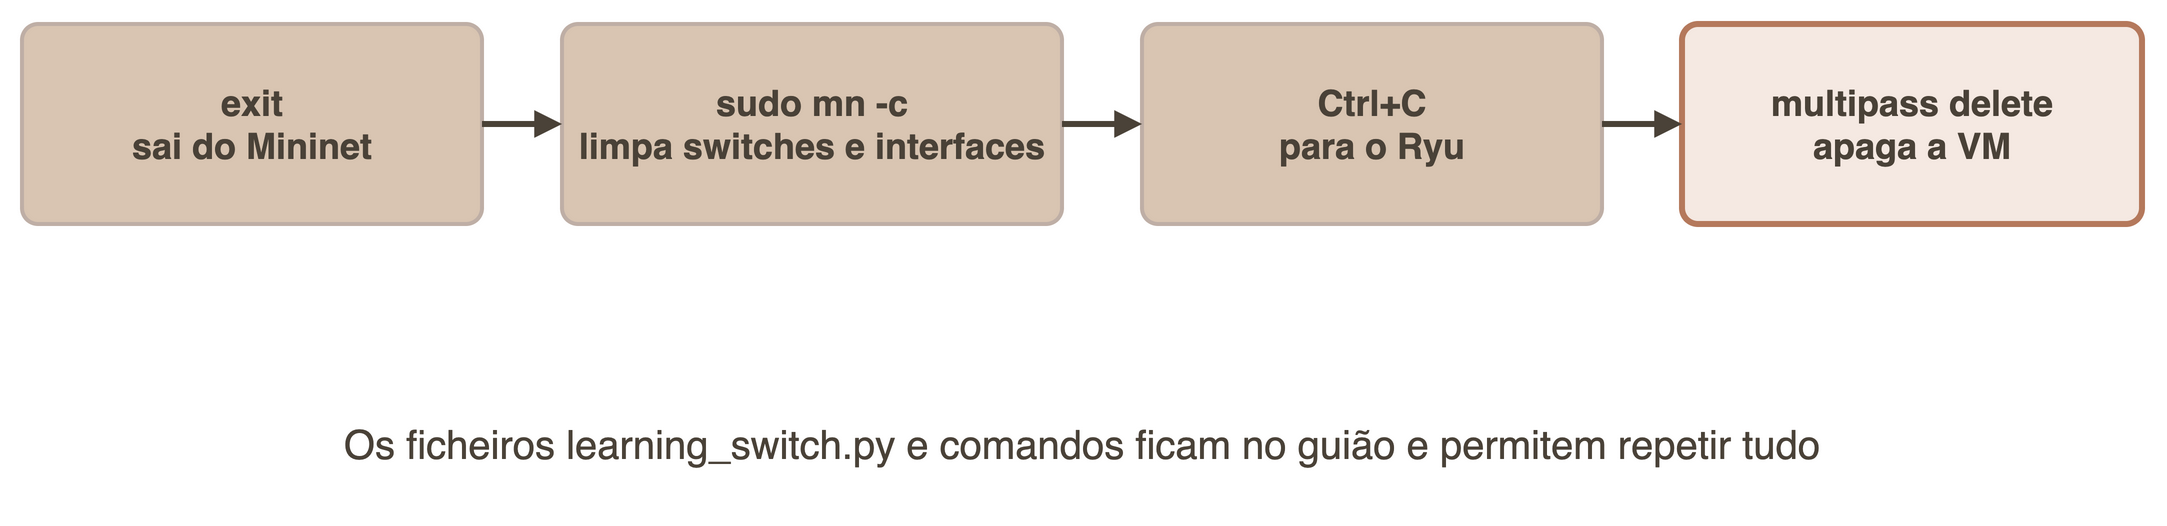
\includegraphics[width=\linewidth]{../Diagramas/g06-limpeza.png}
\end{center}

\begin{leitura}
A sequência da esquerda para a direita corresponde à ordem de execução. Primeiro sai-se do Mininet e limpam-se os switches e as interfaces que ele criou. Depois pára-se o controller. Por fim, a caixa avermelhada apaga a máquina virtual, e com ela tudo o que foi instalado.
\end{leitura}

\subsection*{7.1 Eliminação}

Dentro da máquina virtual:

\begin{terminal}
mininet> exit
sudo mn -c
sudo ip netns del ns1
sudo ip netns del ns2
\end{terminal}

No terminal 1, parar o controller com \cmd{Ctrl+C}. Depois, no computador do aluno, fora da máquina virtual:

\begin{terminal}
exit
multipass delete icn-sdn
multipass purge
\end{terminal}

\subsection*{7.2 Verificação}

\begin{terminal}
multipass list
\end{terminal}

\begin{saida}
No instances found.
\end{saida}

\begin{nota}
Para repetir o laboratório, bastam os comandos do passo 1 e o ficheiro \cmd{learning\_switch.py}. Convém guardá-lo fora da máquina virtual, por exemplo com \cmd{multipass transfer icn-sdn:/home/ubuntu/icn-aula06/learning\_switch.py .} antes de a apagar.
\end{nota}

\clearpage
\section*{Resolução de problemas: consulta rápida}

\renewcommand{\arraystretch}{1.7}
\begin{center}
\small
\begin{tabular}{>{\raggedright\arraybackslash}p{5.6cm} >{\raggedright\arraybackslash}p{9.2cm}}
\toprule
\textbf{Sintoma} & \textbf{Resolução} \\
\midrule
\cmd{multipass: command not found} & Fechar e abrir o terminal. Se persistir, repetir a instalação. \\
\cmd{launch failed} ou VM parada & Libertar memória e repetir. Se existir, \cmd{multipass delete icn-sdn} e \cmd{multipass purge}. \\
Falha ao instalar o Ryu & Instalar \cmd{setuptools==58.2.0} e \cmd{wheel} no ambiente virtual e repetir. \\
\cmd{ALREADY\_HANDLED} no \cmd{ryu-manager} & \cmd{pip install "eventlet==0.30.1"} no ambiente virtual do Ryu. \\
\cmd{Exception: Error creating interface pair} & Executar \cmd{sudo mn -c} e repetir o comando do Mininet. \\
\cmd{RTNETLINK: File exists} (Mininet) & Executar \cmd{sudo mn -c}. Um Mininet anterior ficou a meio. \\
\cmd{pingall} falha com controller ligado & \cmd{ovs-vsctl show} e ler \cmd{is\_connected}. Confirmar o porto com \cmd{ss -lntp}. \\
\cmd{ovs-ofctl} sem resultados & Confirmar \cmd{-O OpenFlow13} e o nome do switch \cmd{s1}. \\
Módulo \cmd{openvswitch} em falta & \cmd{sudo apt install -y linux-modules-extra-\$(uname -r)} ou usar \cmd{-{}-switch ovs,datapath=user}. \\
\cmd{IndentationError} no Ryu & Substituir tabulações por quatro espaços no ficheiro. \\
Primeiro ping lento & Comportamento esperado do modelo reativo. \\
\cmd{Cannot find device veth1} & \cmd{sudo ip netns del ns1}, \cmd{sudo ip netns del ns2} e repetir o passo 6. \\
\bottomrule
\end{tabular}
\end{center}

\section*{Comandos utilizados}

\begin{center}
\small
\begin{tabular}{>{\raggedright\arraybackslash}p{7.2cm} >{\raggedright\arraybackslash}p{7.6cm}}
\toprule
\textbf{Comando} & \textbf{Finalidade} \\
\midrule
\cmd{multipass launch 22.04 -{}-name icn-sdn} & Criar a máquina virtual \\
\cmd{sudo mn -{}-topo single,3 -{}-mac} & Criar três hosts e um switch \\
\cmd{-{}-controller none} & Arrancar o switch sem controller \\
\cmd{-{}-controller remote,ip=...,port=...} & Ligar a um controller externo \\
\cmd{pingall} & Testar a conectividade entre todos os hosts \\
\cmd{ovs-ofctl -O OpenFlow13 dump-flows s1} & Listar a tabela de fluxos \\
\cmd{ovs-ofctl -O OpenFlow13 add-flow s1 ...} & Instalar uma regra \\
\cmd{ovs-ofctl -O OpenFlow13 del-flows s1} & Remover todas as regras \\
\cmd{ovs-vsctl show} & Mostrar bridges, portas e controller \\
\cmd{ryu-manager learning\_switch.py} & Executar o controller \\
\cmd{ip netns add / exec} & Criar e usar um namespace de rede \\
\cmd{ip link add ... type vxlan id 42} & Criar uma interface VXLAN \\
\cmd{tcpdump -ni veth1 udp port 4789} & Capturar tráfego VXLAN \\
\cmd{sudo mn -c} & Limpar switches e interfaces do Mininet \\
\cmd{multipass delete icn-sdn} & Apagar a máquina virtual \\
\bottomrule
\end{tabular}
\end{center}

\section*{Questões de consolidação}

As questões seguintes destinam-se a discussão e não têm de ser entregues.

\begin{enumerate}
  \item Porque é que o \cmd{pingall} falhou no passo 2 e funcionou depois de uma única regra \cmd{NORMAL}? Onde estava o plano de controlo em cada caso?
  \item O controller do passo 3 segue um modelo reativo ou proativo? Justificar com o que se observou no primeiro ping do passo 4.
  \item Que informação usa o controller para escolher a porta de saída, e em que camada do modelo OSI se encontra?
  \item Porque é que a regra de bloqueio prevaleceu sobre a regra de encaminhamento sem alterar o controller?
  \item Qual é o \emph{underlay} e qual é o \emph{overlay} no passo 6? Que parte do pacote é visível para a rede subjacente?
\end{enumerate}

\section*{Síntese}

O laboratório permitiu observar, na prática, as ideias centrais da Aula 06:

\begin{itemize}
  \item Um switch sem regras não encaminha tráfego: o \textbf{plano de dados} depende do \textbf{plano de controlo}.
  \item O \textbf{controller} decide e o switch aplica. A tabela de fluxos é o ponto de contacto entre os dois.
  \item Cada entrada tem \textbf{prioridade}, \textbf{contadores} e \textbf{timeouts}, e é o que permite medir e governar o tráfego.
  \item No modelo \textbf{reativo}, o primeiro pacote de um fluxo vai ao controller, e os seguintes seguem a regra instalada.
  \item Uma \textbf{política} é uma regra mais específica e de maior prioridade, que se sobrepõe ao encaminhamento geral.
  \item Uma rede \textbf{overlay} embrulha o tráfego em UDP, e a rede física vê apenas o \textbf{underlay}.
\end{itemize}

\end{document}
